% !TEX encoding = UTF-8
% !TEX TS-program = pdflatex
% !TEX root = ../tesi.tex

%**************************************************************
\chapter{Messages}
\label{cap:messages}
%**************************************************************

%**************************************************************
\section{Structure of packets}

There is one generic packet that will be exchanged during the client - server communication. We shall call it ``OperationPacket'' and it is made of: \newline{}
\begin{itemize}
	\item AAD (24 bytes)
	\item IV (12 bytes)
	\item PAYLOAD (variable size defined inside the AAD)
	\item TAG (16 bytes)
\end{itemize}
The AAD content is represented in the Table \ref{tab:AAD-content}.
\begin{longtable}{|p{0.4\textwidth}|p{0.2\textwidth}|}
	\caption{AAD content}
	\label{AAD content} 
	\label{tab:AAD-content} \\
	\hline
	\textbf{Content} & \textbf{Size} \\
	\hline
	Operation ID & 4 bytes \\
	\hline
	Message counter & 8 bytes \\
	\hline
	Payload length & 8 bytes \\
	\hline
	Number of Packets & 4 bytes \\
	\hline
\end{longtable}%

An in depth description of every single content of the AAD is necessary:

\begin{itemize}
	\item \textbf{Operation ID}: represents an integer number that will indicate the type of the operation to be done. The values that Operation ID can have will be listed at \ref{tab:operation-ids-list};
	\item \textbf{Message counter}: counter of the number of messages exchanged between server and client, it is used to avoid replay attack and as such must be in sync both client side and server side;
	\item \textbf{Payload length}: the payload length will be variable and this data will be used to know how many bytes to expect as payload;
	\item \textbf{Number of packets}: Some operations will send data in multiple packets, this value is used to know how many packets to expect.
\end{itemize}

\begin{longtable}{|p{0.06\textwidth}|p{0.15\textwidth}|p{0.79\textwidth}|}
	\caption{Operation ID values and description}
	\label{Operation ID list} 
	\label{tab:operation-ids-list} \\
	\hline
	\textbf{Value} & \textbf{Operation} & \textbf{Description} \\
	\hline
	 0 & ACK & Message received, the operation is allowed and can continue \\
	\hline
	 1 & UPLOAD & Client operation used to ask the server for permission to upload a local file to remote \\
	\hline
	 2 & DOWNLOAD & Client operation used to ask the server for permission to download a remote file to local \\
	\hline
	 3 & DELETE & Client operation used to ask the server for permission to delete a remote file \\
	\hline
	 4 & LIST & Client operation used to ask the server the list of remote files  \\
	\hline
	 5 & RENAME & Client operation used to ask the server to rename a remote file \\
	\hline
	 6 & LOGOUT & Client operation used to gracefully close the connection \\
	\hline
	 7 & DONE & Used to communicate that the previous operation has been completed successfully \\
	\hline
	 8 & ABORT & Message received, the operation is not allowed and cannot continue \\
	\hline
	 9 & DATA & The packet contains file data \\
	\hline
\end{longtable}%

\section{Operations} \label{sec:operations}

In this section every operation and its sequence diagram will be discussed and explained.

\subsection{Upload}
\begin{enumerate} 
	\item client, after validating filename, file existance and size, sends OperationPacket with payload made of the filename and AAD made of message counter and: \newline{}
	\begin{itemize}
		\item operation ID = UPLOAD;
		\item number of packets that will be sent to server;
		\item payload length: the size of the filename.
	\end{itemize}
	\item server validates the request checking the filename and if the file does not exists already and sends ACK if valid, otherwise ABORT;
	\item client starts sending in order but asynchronously data packets containing the content of the files;
	\item server reads and validates every packets, checking if they are being received in the correct order. When the server finishes reading all the packets it sends a DONE.

\end{enumerate}

\begin{figure}[!h] 
    \centering 
    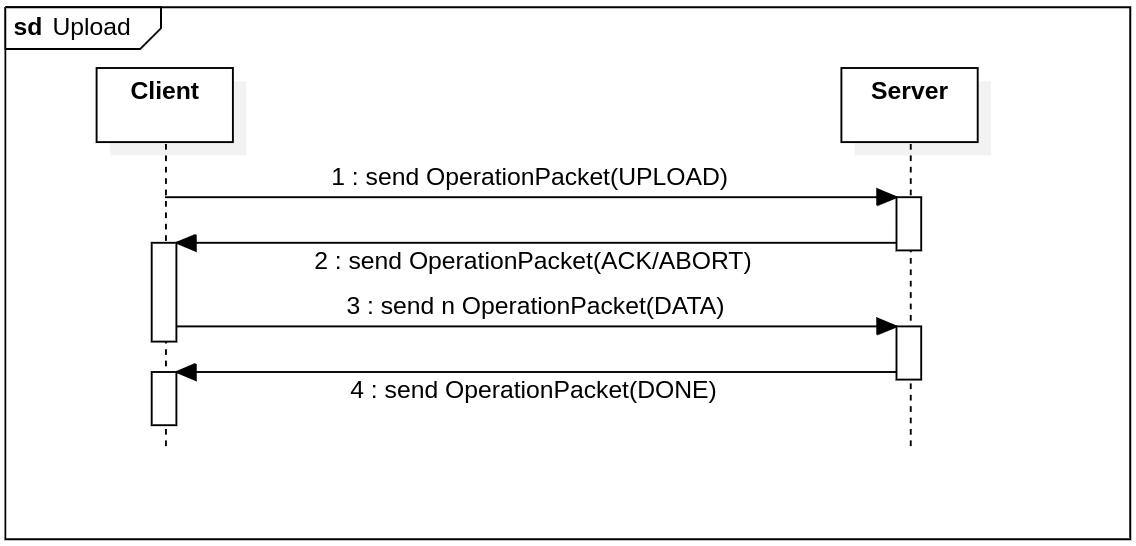
\includegraphics[width=1\columnwidth]{chapter-3/Upload.png} 
    \caption{Upload operation.}
    \label{fig:upload_operation}
\end{figure}

\newpage{}

\subsection{Download}
\begin{enumerate}
	\item client, after validating filename and file existance, sends OperationPacket with payload made of the filename and AAD made of message counter and: \newline{}
	\begin{itemize}
		\item operation ID = DOWNLOAD;
		\item payload length: the size of the filename.
	\end{itemize}
	\item server validates the request checking filename and if the file exists and sends ACK if valid, otherwise ABORT;
	\item client sends ACK;
	\item server starts sending in order but asynchronously data packets containing the content of the files;
	\item client reads and validates every packets, checking if they are being received in the correct order. When the client finishes reading all the packets it sends a DONE.
\end{enumerate}

\begin{figure}[!h] 
    \centering 
    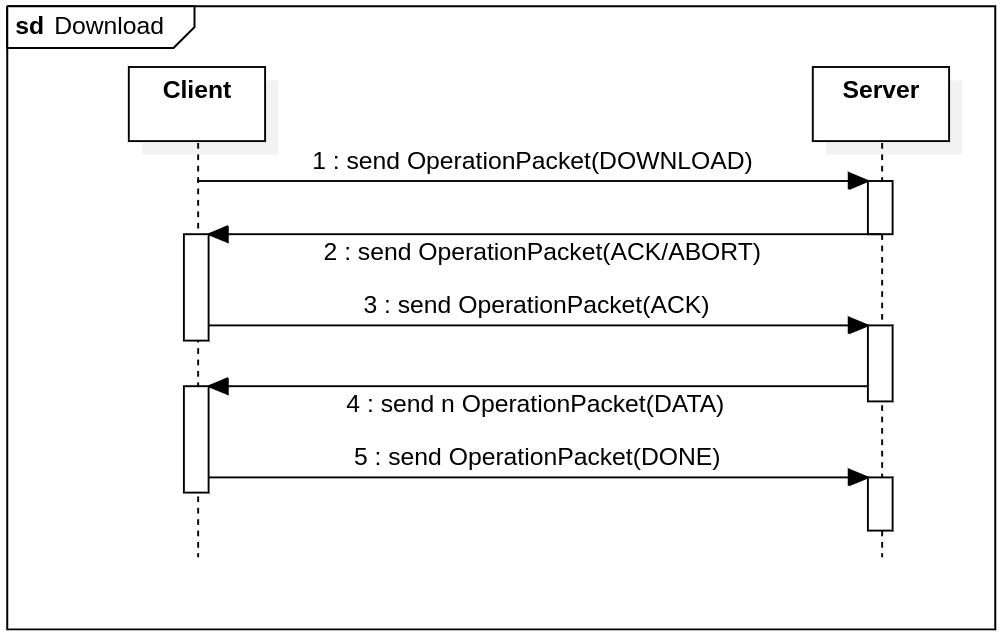
\includegraphics[width=1\columnwidth]{chapter-3/Download.png} 
    \caption{Download operation.}
    \label{fig:download_operation}
\end{figure}
\newpage{}
\subsection{List}
\begin{enumerate}
	\item client sends OperationPacket LIST;
	\item server sends OperationPacket DATA containing all the filenames found and validated by the server on the remote folder, separated by ','. Ex: file1,file2,file3 ;
	\item client reads the OperationPacket and splits the received payload in strings, validates them and display them to console.
	
\end{enumerate}
\begin{figure}[!h] 
    \centering 
    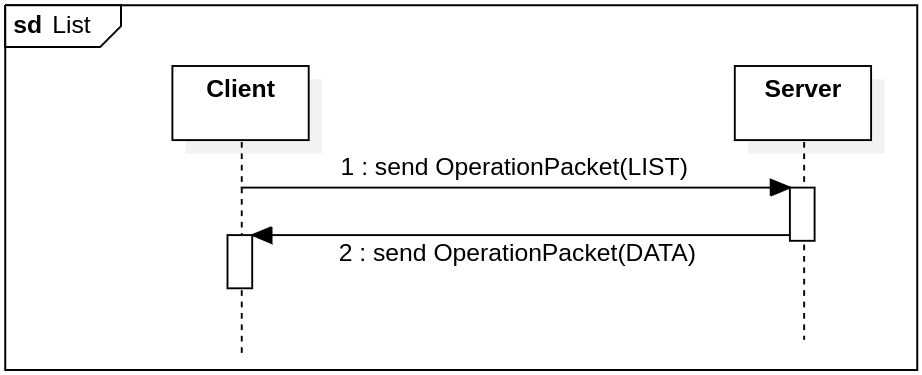
\includegraphics[width=1\columnwidth]{chapter-3/List.png} 
    \caption{List operation.}
    \label{fig:list_operation}
\end{figure}

\subsection{Delete}
\begin{enumerate}
	\item client inputs a filename, validates the input and if valid checks for client confirmation of this destructive operation. The check is made client side because, if someone modified the client source code, then it would be as trivial to skip the client side check as it would to send an automatic ACK message after the server asks for confirmation. This means that a server side check will not provide benefit nor in security nor in speed while putting the check client side the security will be the same but sending useless packets will be avoided;
	\item client sends OperationPacket DELETE with payload containing filename;
	\item server validates the request checking filename and if the file exists and delete file and sends DONE if valid, otherwise ABORT;
\end{enumerate}

\begin{figure}[!h] 
    \centering 
    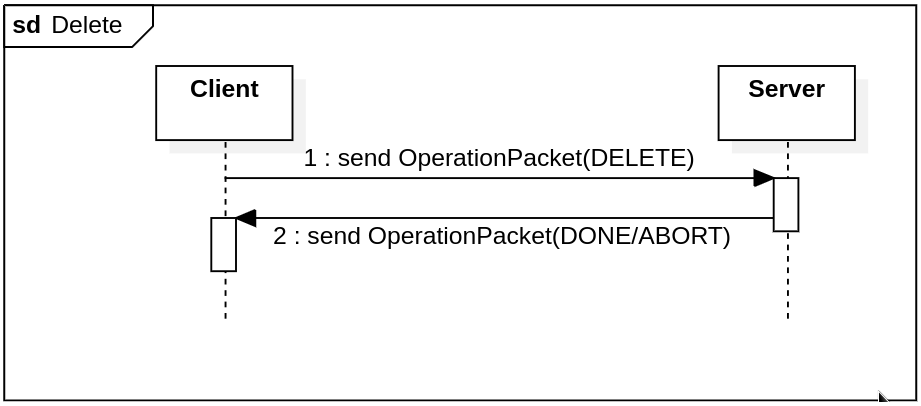
\includegraphics[width=1\columnwidth]{chapter-3/Delete.png} 
    \caption{Delete operation.}
    \label{fig:delete_operation}
\end{figure}

\subsection{Rename}
\begin{enumerate}
	\item client first inputs the file to rename and after that the name that he wants to rename it to. Every step of the input is validated;
	\item client sends OperationPacket RENAME containing the two filenames as payload, separated by ','. Ex: fileold.example,filenew.txt ;
	\item server reads the OperationPacket and splits the received payload in two strings, old and new name. It validates the two, checks if the old filename exists in the remote folder and then renames it to the desired new name. If this was successful sends DONE, otherwise ABORT.
\end{enumerate}

\begin{figure}[!h] 
    \centering 
    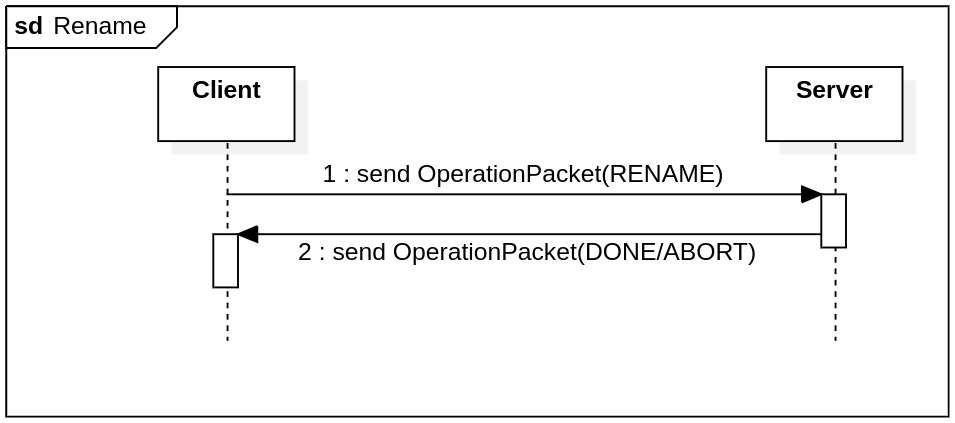
\includegraphics[width=1\columnwidth]{chapter-3/Rename.png} 
    \caption{Rename operation.}
    \label{fig:rename_operation}
\end{figure}
\newpage{}
\subsection{Logout}
\begin{enumerate}
	\item client sends OperationPacket LOGOUT;
	\item server answers with OperationPacket ACK;
	\item client asks the user to confirm the operation;
	\item if the operation was confirmed sends DONE to server and closes the connection, otherwise ABORT;
	\item server reads the OperationPacket and if DONE it closes the connection on its part, otherwise it ignores the previous request and keeps the connection going.
\end{enumerate}


\begin{figure}[!h] 
    \centering 
    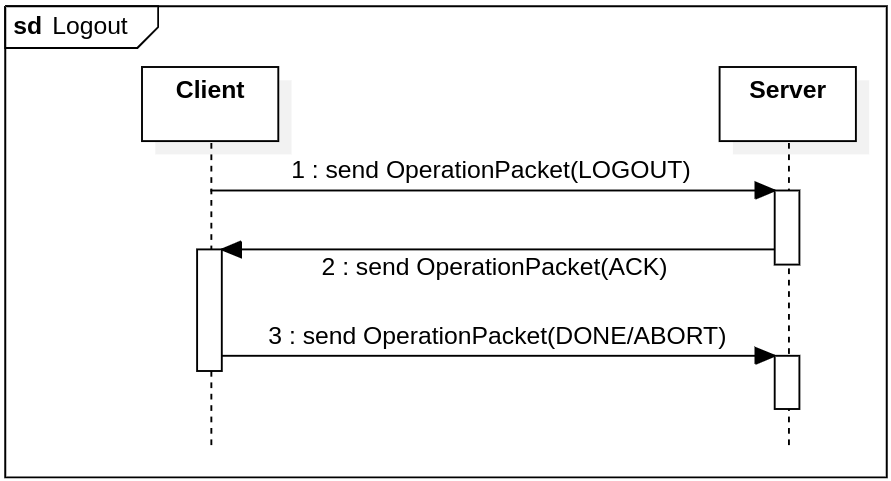
\includegraphics[width=1\columnwidth]{chapter-3/Logout.png} 
    \caption{Logout operation.}
    \label{fig:logout_operation}
\end{figure}
